\chapter{Simulation Environment}
\begin{figure}[h!]
\centering
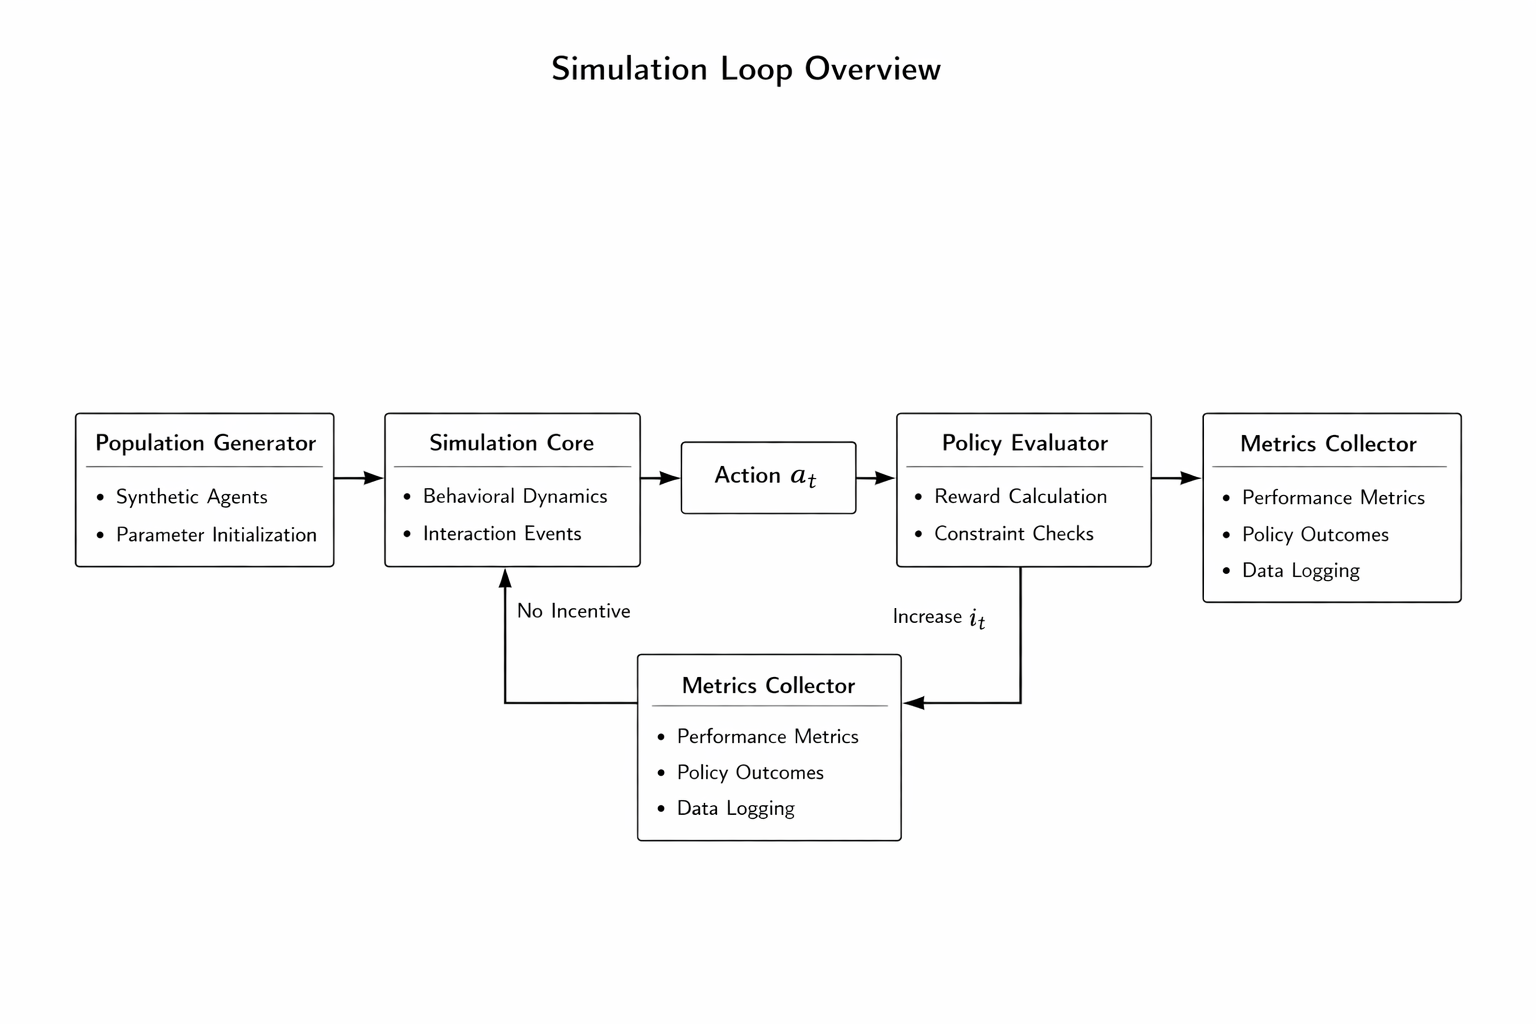
\includegraphics[width=0.9\textwidth]{figures/simulation_loop.png}
\caption{Simulation loop used to evaluate BED policies across heterogeneous synthetic populations.}
\label{fig:simulation_loop}
\end{figure}
The simulation environment provides a controlled setting for evaluating the
Behavioral Engine for Demand (BED) under realistic behavioral dynamics and
operational constraints. It enables experimentation with different incentive
policies, behavioral parameters, and budget levels without requiring access to
real-world user data. This chapter describes the architecture, components, and
workflow of the BED v3 simulation environment.

\section{Overview}

The simulation environment integrates four core modules:

\begin{enumerate}
    \item \textbf{Behavioral State Engine}: Implements the recency, habit,
    responsiveness, and incentive decay dynamics described in Chapter 4.
    \item \textbf{Hazard Model}: Computes event probabilities using a logistic
    hazard function.
    \item \textbf{CMDP Policy Engine}: Selects incentive actions under budget
    constraints.
    \item \textbf{Experiment Runner}: Executes multi-step simulations and logs
    behavioral trajectories.
\end{enumerate}

These modules correspond directly to the Python files in the simulation
directory: \texttt{bed\_engine.py}, \texttt{hazard\_model.py},
\texttt{cmdp\_solver.py}, and \texttt{run\_simulation.py}.

\section{Synthetic Population}

The simulation environment generates a synthetic population of users, each with
unique behavioral parameters. This allows BED to evaluate policy performance
across heterogeneous responsiveness levels. Each simulated user is initialized
with:

\begin{itemize}
    \item a recency value $r_0$,
    \item a habit value $h_0$,
    \item a responsiveness parameter $\rho$,
    \item an initial incentive decay state $\Delta_0$,
    \item a last incentive magnitude $I_{-1}$.
\end{itemize}

Responsiveness values may be drawn from a distribution (e.g., beta or normal)
to reflect population heterogeneity.

\section{Behavioral State Engine}

The behavioral state engine updates user state at each time step according to
the rules defined in Chapter 4. The Python implementation in
\texttt{bed\_engine.py} mirrors these update equations:

\begin{itemize}
    \item recency increases unless an event occurs,
    \item habit decays or strengthens depending on engagement,
    \item incentive decay increases unless a new incentive is delivered,
    \item the last incentive magnitude is updated when an action is taken.
\end{itemize}

This ensures that the simulation environment faithfully reproduces the BED
behavioral model.

\section{Hazard Model}

The hazard model computes the probability of an event at each time step:


\[
P(\text{event}_t = 1 \mid s_t) =
\sigma\left(
\beta_0
+ \beta_r r_t
+ \beta_h h_t
+ \beta_\rho \rho_t
+ \beta_I I_{t-1} e^{-\lambda \Delta_t}
\right).
\]



The implementation in \texttt{hazard\_model.py} uses a logistic function to
compute this probability. The hazard model is responsible for introducing
stochasticity into the simulation: even users with identical states may behave
differently due to randomness in event outcomes.

\section{CMDP Policy Engine}

The CMDP policy engine selects actions based on:

\begin{itemize}
    \item the current behavioral state,
    \item the remaining budget,
    \item the cost of delivering an incentive,
    \item fairness or eligibility constraints (if enabled).
\end{itemize}

The public-safe implementation in \texttt{cmdp\_solver.py} uses a simple
threshold-based policy derived from the Lagrangian relaxation described in
Chapter 5. More advanced policies (e.g., value iteration, policy gradient
methods) can be substituted without modifying the simulation architecture.

\section{Experiment Runner}

The experiment runner orchestrates the simulation. The implementation in
\texttt{run\_simulation.py} performs the following steps:

\begin{enumerate}
    \item Initialize the behavioral state.
    \item For each time step:
    \begin{enumerate}
        \item compute event probability using the hazard model,
        \item sample event occurrence,
        \item select an action using the CMDP policy engine,
        \item update the behavioral state,
        \item log the state, action, and event.
    \end{enumerate}
\end{enumerate}

The output is a trajectory of behavioral states, actions, and outcomes that can
be used for analysis and visualization.

\section{Configuration File}

Simulation parameters are stored in a YAML configuration file
(\texttt{config.yaml}). These include:

\begin{itemize}
    \item number of simulation steps,
    \item hazard model coefficients,
    \item habit retention and reinforcement parameters,
    \item incentive decay rate,
    \item CMDP budget and cost parameters.
\end{itemize}

This design allows researchers to modify simulation settings without editing
code, supporting reproducibility and parameter sweeps.

\section{Metrics and Evaluation}

The simulation environment computes several key metrics:

\begin{itemize}
    \item \textbf{engagement rate}: proportion of time steps with events,
    \item \textbf{habit trajectory}: evolution of $h_t$ over time,
    \item \textbf{budget utilization}: fraction of budget spent,
    \item \textbf{policy efficiency}: events per incentive delivered,
    \item \textbf{responsiveness stratification}: performance across user types.
\end{itemize}

These metrics allow for comprehensive evaluation of incentive policies.

\section{Scalability and Extensibility}

The simulation environment is designed to be:

\begin{itemize}
    \item \textbf{modular}: components can be replaced independently,
    \item \textbf{scalable}: supports large synthetic populations,
    \item \textbf{extensible}: new behavioral variables or policy engines can be
    added with minimal changes.
\end{itemize}

This flexibility supports ongoing research and future extensions of BED.

\section{Summary}

The simulation environment provides a rigorous and flexible platform for
evaluating BED policies. It integrates behavioral modeling, hazard-based event
prediction, CMDP optimization, and experiment execution into a unified system.
The next chapter describes the prototype architecture that enables real-world
deployment and experimentation.
